\section{LSTM}
\begin{frame}[fragile]
  \frametitle{LSTM}
  ~
\end{frame}

\begin{frame}[fragile]
  \frametitle{RNN: 循环神经网络}

  人类针对每个问题的思考,不会完全的从头开始思考,例如阅读文章,会根据已经阅读过
  的内容来对后面的内容进行理解。

  RNN允许信息持续存在

  
\end{frame}

\begin{frame}[fragile]
  \frametitle{RNN}
  \begin{columns}[T]
    \column{0.4\textwidth}
    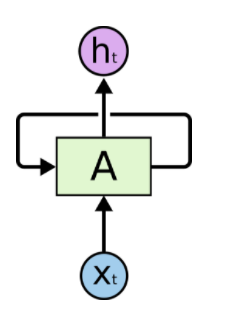
\includegraphics[width=0.6\textwidth]{figures/RNN-1.png}

    \column{0.6\textwidth}
    一组神经网络$A$接收某些输入$x_t$,并输出一个值$h_t$。 允许信息从网络的一个步
    骤循环传递到下一个。

    将循环展开会发生什么?(示意如下)
  \end{columns}

  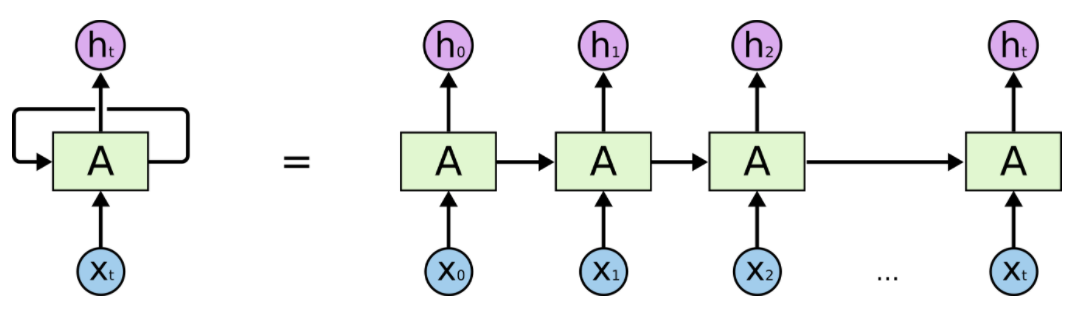
\includegraphics[width=0.9\textwidth]{figures/RNN-2.png}
\end{frame}

\begin{frame}[fragile]
  \frametitle{RNN}
  \begin{itemize}
  \item 循环神经网络与序列和列表密切相关。
  \item RNN应在语音识别、语言建模、翻译,图像字幕等各种问题上取得了巨大成功。
  \item The Unreasonable Effectiveness of Recurrent Neural Networks

    From: \url{http://karpathy.github.io/2015/05/21/rnn-effectiveness/}     
  \end{itemize}
\end{frame}


\begin{frame}[fragile]
  \frametitle{Reference}
  \begin{itemize}
  \item https://www.jianshu.com/p/4b4701beba92
  \end{itemize}
\end{frame}